\clearpage
\section{Implementácia}\label{sec:programming}

Aplikácia pozostáva z dvoch častí a to \textbf{časť umelej inteligencie} a \textbf{hra}.
V časti umelej inteligencie sa vytvára a trénuje umelá neurónová sieť, v hernej časti sa dá hra ovládať pomocou
ovládača od hernej konzoly Xbox a zobrazená je v prostredí \emph{Cave}.

\subsection{Unity}\label{subsec:unity}
Samotná ovládacia časť (hra) je vytvorená v prostredí Unity verzie 2019.2.17f1.
Pozostáva z niekoľkých modulov:

\textbf{Scény} sú v rámci unity kontajnery pre herné objekty (napr. 3D model) v rámci jedného logického celku.
Scéna je v klasických hrách ekvivalentom levelu alebo prostredia, v ktorom sa hráč nachádza.
V hre sa nachádzajú dve scény: scéna pre hlavné menu a scéna pre hraciu plochu.

Ďalšou dôležitou časťou sú \textbf{vopred pripravené súbory} (angl. a ďalej len \emph{prefabs}), čo sú v podstate herné
objekty, ktoré sú zložené z už existujúcich herných objektov pre účely znovupoužitia.
Vytvorené sú prefabs pre tlačidlo v menu, posuvník v menu (pre výber napr. veľkosti hracieho priestoru), oddeľovač
buniek v hracom priestore, bunku v hracom priestore a znaky \textbf{X} a \textbf{O} vytvorené pre 3D priestor.

\textbf{Skripty} sú funkčnou časťou celej aplikácie.
Unity má veľké množstvo skriptov už vopred pripravených, no pre konkrétne využitie je vo väčšine prípadov nutné si
vytvoriť vlastné skripty.
V hre je ich použitých 10:
\begin{enumerate}
    \item \emph{BoardOperations} obsahuje operácie pre hraciu plochu ako napr. nájdenie víťazného hráča
    \item \emph{ButtonController} ovláda všeobecne tlačidlá v hlavnom menu
    \item \emph{Cell} skript priradený pre jednu bunku v hracej ploche
    \item \emph{Focusable} akýkoľvek prvok v hlavnom menu, na ktorý sa dá "pozrieť"
    \item \emph{GameController} ovláda celý proces v rámci hry
    \item \emph{Grid} je kontajner pre herný priestor
    \item \emph{HudController} ovláda prvky v menu
    \item \emph{PlayerController} obsahuje funkcie pre pohyb hracieho priestoru v zornom poli hráča
    \item \emph{SliderItemController} - posuvník v menu
    \item \emph{BuildScript} spúšťa zostavenie spustiteľného súboru pre platformu Windows
\end{enumerate}

V ostatných súboroch sa nachádzajú stiahnuté \textbf{3D súbory} a \textbf{knižnice}, \textbf{materiály} pre 3D objekty
a \textbf{font} pre písmo v menu.
Zvyšné súbory sú generované vývojovým prostredím.

\begin{figure}[H]
    \centering
    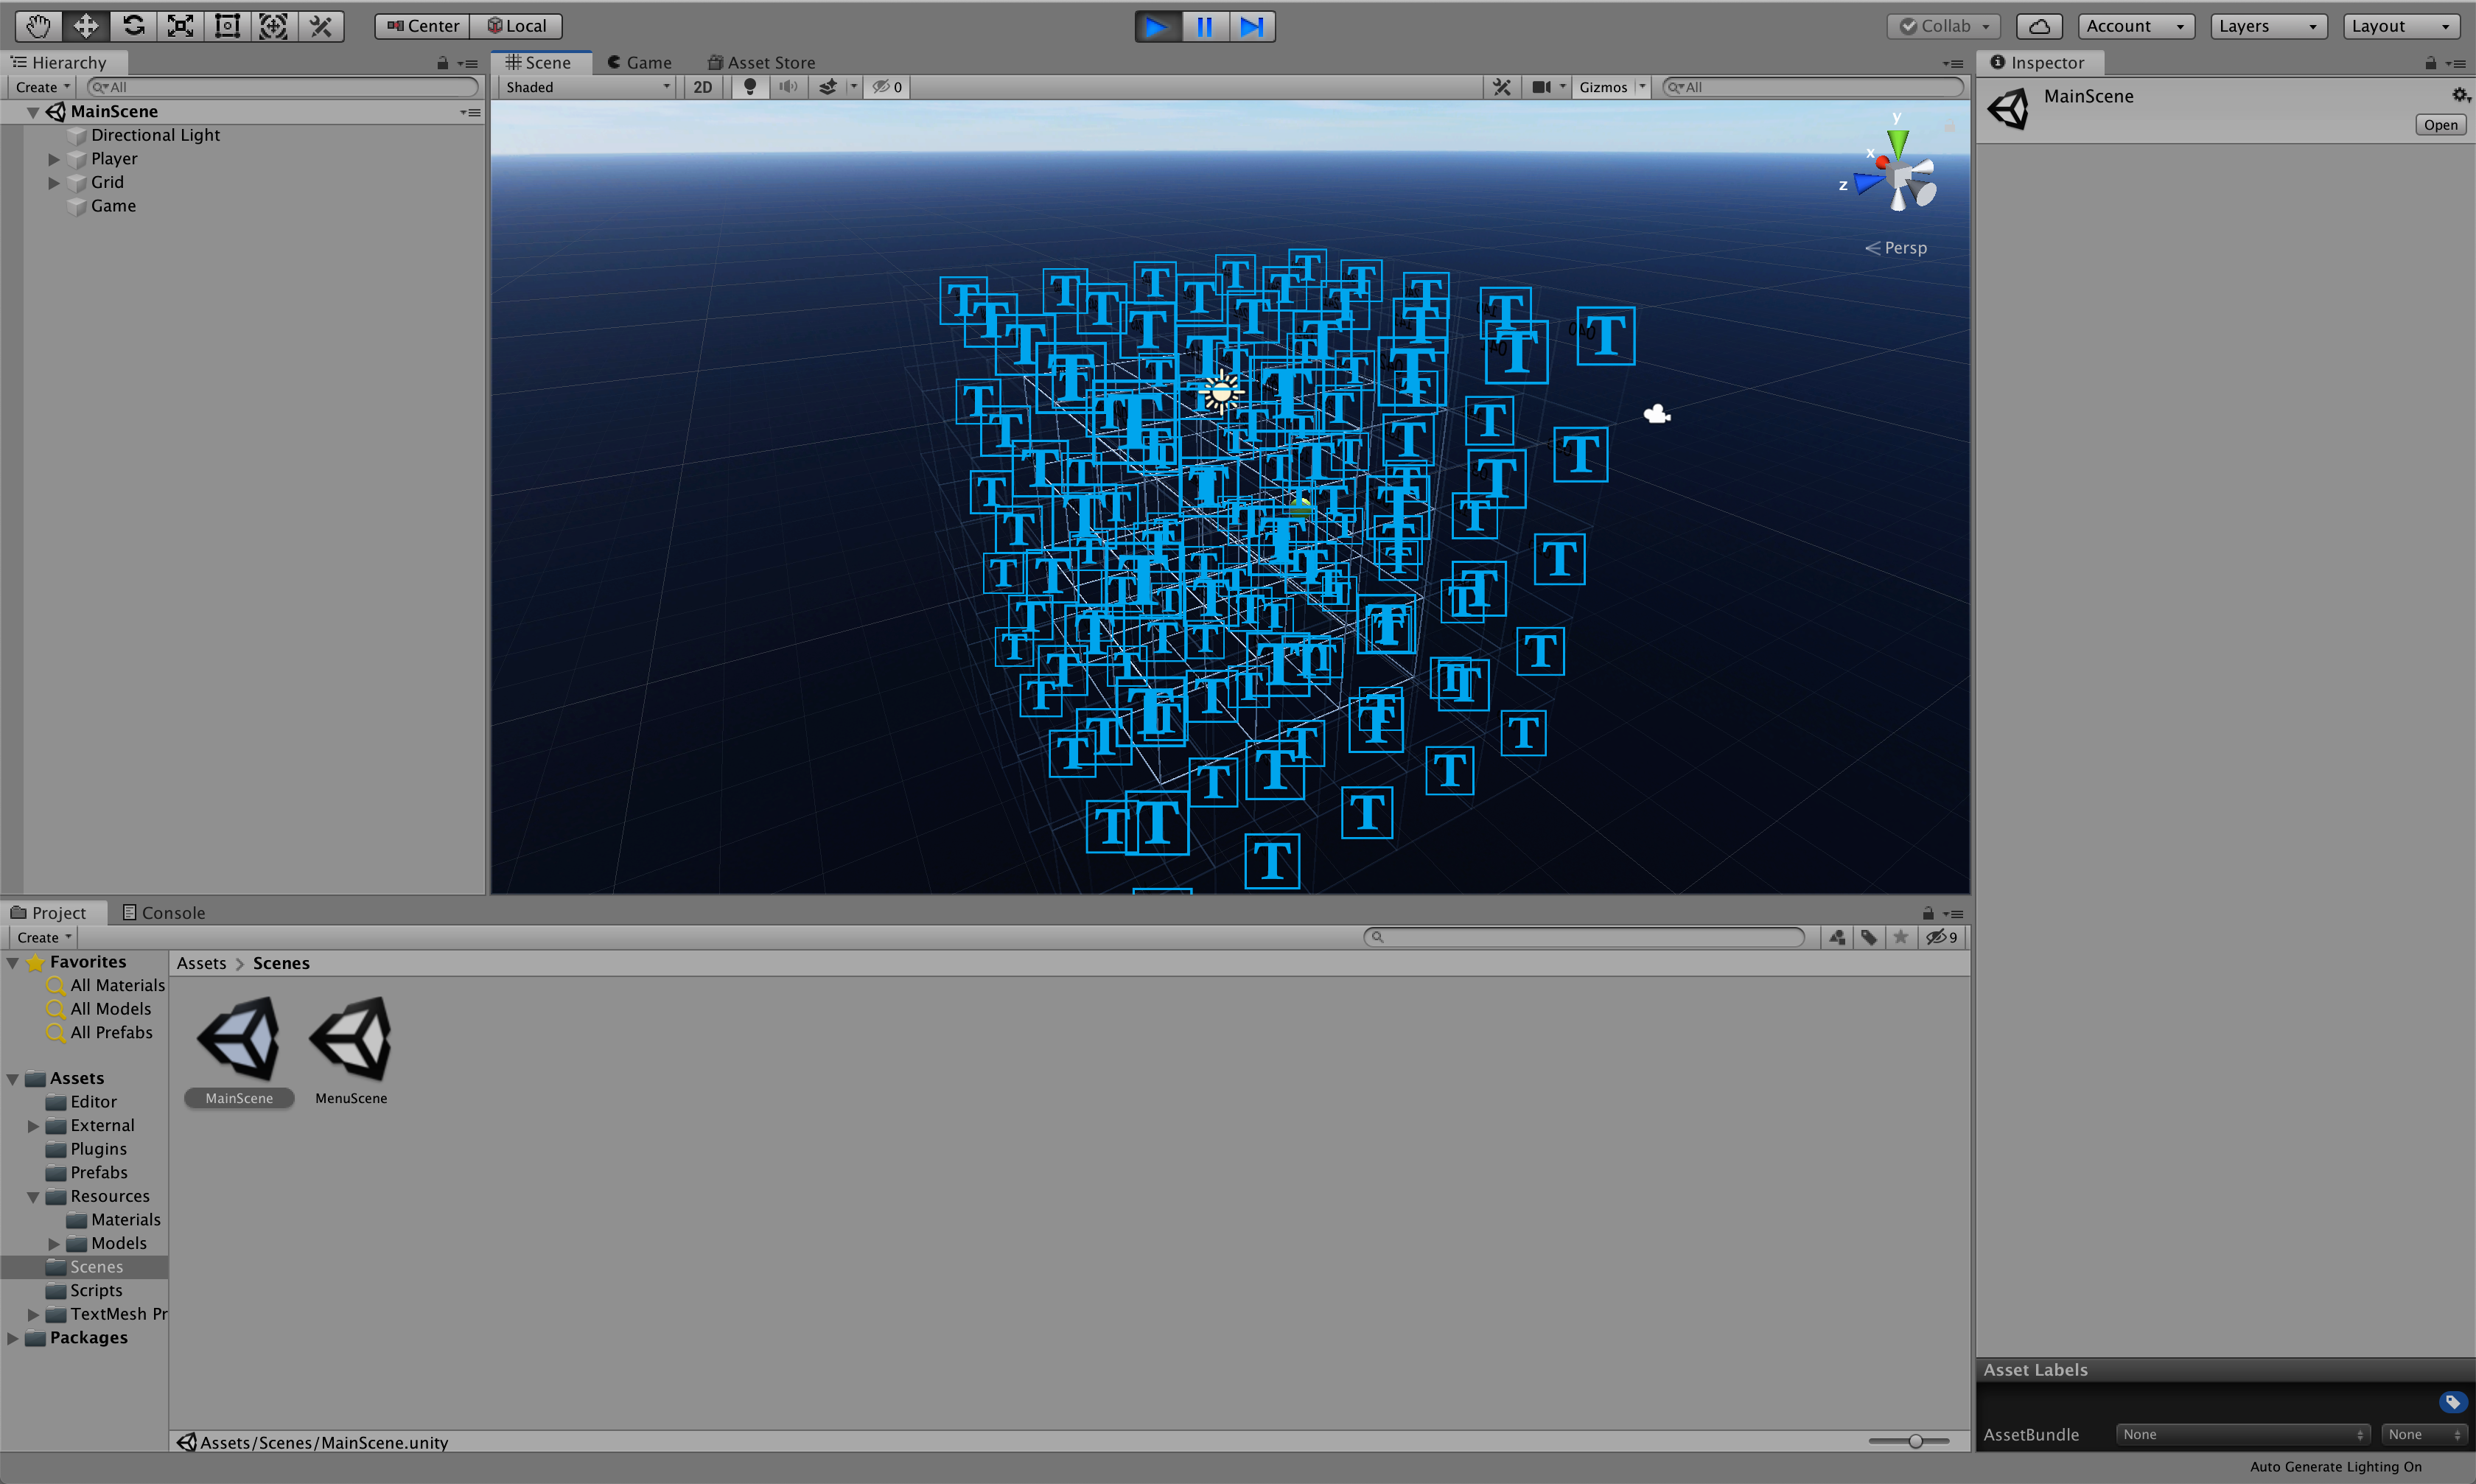
\includegraphics[width=0.5\textwidth]{images/unity.png}
    \caption{Prostredie unity}
\end{figure}\label{figure:unity}

\subsubsection{Prostredie Cave}
Unity pracuje najmä s prostredím \textbf{KAVE} (skr. Kinect Cave) a teda už z názvu vyplýva, že celý systém ovládania
je založený na Microsoft Xbox Kinect.

\subsection{Vývojové prostriedky pre umelú inteligenciu}\label{subsec:dev-tools-for-ai}
python apod
\subsection{Prepojenie umelej inteligencie s prostredím}\label{subsec:connection}

\subsection{Príručky}\label{subsec:helpers}
\subsubsection{Programátorská príručka}
\subsubsection{Užívateľská príručka}
\clearpage